%% Auto-generated from paper_template.tex by 10_build_paper.py; every number is read from discovery_results.json.
\documentclass[aps,prd,twocolumn,superscriptaddress,nofootinbib,floatfix,10pt]{revtex4-2}
\usepackage{amsmath,amssymb,graphicx,booktabs,array}
\usepackage[colorlinks=true,allcolors=blue]{hyperref}
\newcommand{\eps}{\varepsilon}
\newcommand{\lC}{\lambda_C}
\newcommand{\MPl}{M_{\rm Pl}}
\begin{document}

\title{Beyond the static Einstein--Euler--Heisenberg description of an extreme electric field:\\ a formally verified validity map for discharge and trapping}

\author{\'Alvaro L\'opez Almeida}
\date{\today}

\begin{abstract}
We ask what lies beyond the point where the static, quartic-truncated Einstein--Euler--Heisenberg (EEH) description of a point-like electric charge breaks down ($\eps\equiv eE/m_e^2\gtrsim 1$, $r\lesssim\lC$), and whether QED can act as a ``universal quantum censor'' that prevents the gravitational collapse of the field. Every equation used is derived or checked with a computer algebra system (⟦meta.n_gates⟧ gates, ⟦meta.n_negative_controls⟧ of them negative controls that must fail on altered models). We find: (i) the exact one-loop (proper-time) real part does not saturate the field; it reproduces Reissner--Nordstr\"om with a running charge, whereas the quartic truncation and a matched Born--Infeld model yield a spurious single Schwarzschild-like horizon; the dominant-energy condition is violated for $\eps>$⟦branch_A.energy_conditions_qed.DEC_onset_eps_exact|.5f⟧ with relative margin $\to-\alpha/3\pi$ (the one-loop trace anomaly). (ii) The condition $\theta_+=0\Leftrightarrow 2GM_{\rm MS}=R$, the decomposition $M_{\rm ADM}=M_{\rm MS}(R)+U_C(R)$ and the exact cancellation of the electrostatic energy are derived inside the pipeline for time-symmetric spherical data, together with the exact one-loop correction to $U_C$. (iii) A Pauli-blocked Markov kinetic model keeps $0\le f\le \tfrac12$ and gives $\omega_p=$⟦branch_B2.scaling.omega_over_esqrtx0.2|.3f⟧$\,e\sqrt{eE_0}$; replacing the Markov ansatz by the exact Bloch--Bogoliubov equations coupled to Maxwell's equation (the normalization of the coupling is fixed by a Landau--Zener test) lets the occupation reach $f_{\max}=$⟦branch_B3.exact_sweep.100.fmax|.4f⟧, advances the first field zero by ⟦branch_B3.pct_tau0_shift_1000|.0f⟧ per cent, raises the plasma frequency to $\omega_p=$⟦branch_B3.scaling.omega_over_esqrtx0.3|.3f⟧$\,e\sqrt{eE_0}$, and shows that the pairs form a collinear gas with $\langle w_\parallel\rangle=$⟦branch_B3.exact_sweep.1000.w_pl_avg_last_period|.2f⟧ rather than $\tfrac13$, with energy conserved to ⟦#branch_B3.max_energy_err|.1e⟧. (iv) The ratio of the discharge time to the free-fall time obeys $\tau_{\rm dis}/\tau_{\rm ff}=(r_0^*/r_0)^{1/2}$ with $r_0^*$ independent of the number of charges $N$, and a quantitative $(N,r_0)$ phase map is given.  (v) Without time symmetry, the Misner--Sharp balance $\partial_tM_{\rm MS}=-4\pi r^2F_{\rm flux}$ is derived and the internal field-to-plasma conversion is shown to leave $M_{\rm MS}$ unchanged; a 1+1D solver of the discharge of a charged ball in general relativity shows that the plasma leaving through the surface removes only a fraction ⟦branch_C2.weak_gravity_F.inst.f_esc_interior|.2f⟧ of the interior field energy while the ingoing half of the plasma converted outside adds $⟦branch_C2.inflow_over_leak|.1f⟧$ times more, so the net effect is a gain; the dynamics shifts the critical mass by less than ⟦branch_C2.threshold_range_pct|.1f⟧ per cent, and the horizon boundary is set instead by the static interior field energy, which places the shell curve $r_s(N)$ inside an initial apparent horizon for $N>$⟦#branch_C2.N_A_staticcurve_enters_initial_horizon|.1e⟧. Several ingredients are known results that we re-derive and verify; Sec.~\ref{sec:attrib} separates them from what is specific to this work, and Sec.~\ref{sec:limits} states the regimes where the model is not controlled.
\end{abstract}

\maketitle

\section{Introduction}\label{sec:intro}
The Euler--Heisenberg (EH) effective action \cite{heisenberg1936,weisskopf1936,schwinger1951} coupled to Einstein gravity has been used to study QED corrections to charged black holes in its quartic truncation \cite{yajima2001,ruffini2013}. Its validity requires $\eps\ll1$, and for a point charge $Q=Ne$ the static field reaches $\eps=1$ at $r_\eps=\sqrt{N\alpha}\,\lC$, long before any horizon unless $N\gtrsim N_{\rm crit}=\MPl^2/m_e^2\simeq$⟦#branch_C.critical.N_crit|.2e⟧. Beyond that point two qualitatively different effects matter: nonperturbative vacuum pair creation, which discharges the field on plasma time scales \cite{kluger1991,kluger1992,kluger1998,ruffini2010,gelis2016}, and the gravitational response, which depends on whether a trapped surface can exist at all. The loss of charge by black holes through a Schwinger-type mechanism goes back to Gibbons \cite{gibbons1975}, and the structure of charged thin-shell collapse to Israel, Boulware and Bekenstein \cite{boulware1973,bekenstein1971}.

\textbf{Aim and scope.} We do not claim a new law of nature. We build a reproducible, formally gated computation that (a) quantifies where the quartic EEH extrapolation is qualitatively wrong, (b) re-derives the trapping criterion without invoking external theorems, (c) extends the pair-plasma back-reaction through several field reversals with Pauli blocking, and (d) assembles the resulting scales in one phase map. The pipeline (Appendix~\ref{app:pipeline}) executes symbolic derivations (SymPy), adaptive numerical integrations with independent cross-checks, and negative controls; it fails if any gate fails. All numbers quoted below are read automatically from the pipeline output.

\section{Static nonlinear electrodynamics coupled to gravity}\label{sec:static}
\subsection{Reduction for an arbitrary $\mathcal L(E)$}
For the static spherical ansatz $ds^2=-f\,dt^2+dr^2/g+r^2d\Omega^2$, $A=\Phi(r)\,dt$, a purely electric field $E=\sqrt{g/f}\,\Phi'$ and any Lagrangian $\mathcal L(X)$, $X=F_{\mu\nu}F^{\mu\nu}=-2E^2$, the stress tensor derived from the full tensor expression obeys
\begin{align}
T^t{}_t&=T^r{}_r=-\rho,\quad \rho=E\mathcal L'-\mathcal L,\quad T^\theta{}_\theta=\mathcal L,\label{eq:T}\\
r^2\mathcal L'(E)&=Q/4\pi,\qquad f=g=1-\frac{2Gm(r)}{r},\quad m'=4\pi r^2\rho,\label{eq:red}
\end{align}
and $\rho'=-(2/r)(\rho+p_\perp)$ holds identically (gates S1--S4; the control C1 with $p_\perp=\mathcal L/2$ is detected). For Maxwell, $\rho=E^2/2$; for the quartic EH term, $\mathcal L=E^2/2+4cE^4$ with $c=\alpha^2/90\,m_e^4$.

\subsection{One-loop proper-time Lagrangian and strong-field behaviour}
For purely electric fields the spinor one-loop correction is
\begin{equation}
\mathcal L_1(x)=-\frac{1}{8\pi^2}\!\int_0^\infty\!\frac{ds}{s^3}e^{-s}\Big[xs\cot(xs)-1+\tfrac{(xs)^2}{3}\Big],\ \ x=e E,
\end{equation}
evaluated on the ray $s=\rho e^{-i\pi/4}$ because the poles of $\cot$ lie on the real axis. The real part is the effective Lagrangian; the imaginary part reproduces the Schwinger series $\mathrm{Im}\,\mathcal L_1=\frac{x^2}{8\pi^3}\sum_n n^{-2}e^{-n\pi/x}$ to a relative error of ⟦#branch_A.numerics.im_series_max_relerr|.1e⟧ (gate N1), and for $\eps\ll1$ it matches $4cE^4$ with $\mathcal L_1/(4cE^4)-1\propto\eps^{⟦branch_A.numerics.small_eps_slope|.2f⟧}$ (N2; the Taylor coefficient is checked symbolically, S6).

At strong field the expansion is logarithmic, in agreement with the known renormalization-group structure \cite{ritus1975,dunne2004}:
\begin{equation}
\mathcal L=\frac{E^2}{2}\Big[1-\frac{\alpha}{3\pi}\big(\ln\eps+3K\big)\Big],\quad K=⟦branch_A.Landau.K_asym|.4f⟧,
\label{eq:log}
\end{equation}
where the coefficient is verified symbolically (S7) and the slope $d(\mathcal L_1/x^2)/d\ln x=⟦#branch_A.numerics.log_slope_fit|.8e⟧$ agrees with $-1/24\pi^2=⟦#branch_A.numerics.log_slope_expected|.8e⟧$ (N3). The pole of Eq.~(\ref{eq:log}) sits at $\log_{10}\eps_L=⟦branch_A.Landau.log10_eps_L|.1f⟧$, i.e.\ $\mu_L=\sqrt{eE}\approx10^{⟦audit_checks.landau_scale_GeV_log10|.1f⟧}$~GeV, consistent with the usual Landau scale of QED, whereas the Planck density corresponds to $\log_{10}\eps_{\rm Pl}=⟦branch_A.Landau.log10_eps_Planck|.1f⟧$. This holds \emph{at one loop}: the Ritus--Narozhny conjecture, that each loop in a strong field costs $\alpha\chi^{2/3}$ and perturbation theory fails for $\chi\gtrsim\alpha^{-3/2}\simeq⟦audit_checks.ritus_narozhny_chi_threshold|.0f⟧$ \cite{fedotov2017,fedotov2023}, would invalidate all one-loop statements far below $\eps_L$; its applicability to a pure electric field is not established here.

\subsection{Energy conditions and the trace anomaly}
WEC and NEC hold for the one-loop Lagrangian up to $\eps=10^{40}$ (the minima of $\rho/E^2$ and $ED/E^2$ are ⟦branch_A.energy_conditions_qed.WEC_rho_min|.3f⟧ and ⟦branch_A.energy_conditions_qed.NEC_ED_min|.3f⟧, gate N7), and $\mathcal L>0$ (SEC) until the pole (N8). The dominant energy condition $\rho\ge|p_\perp|$ requires $ED-2\mathcal L\ge0$, and SymPy establishes the identity (gate S10)
\begin{equation}
ED-2\mathcal L=x\mathcal L_1'-2\mathcal L_1=x^3\frac{d}{dx}\Big(\frac{\mathcal L_1}{x^2}\Big).
\end{equation}
Hence the DEC is violated exactly where $\mathcal L_1/x^2$ decreases, i.e.\ for $\eps>$⟦branch_A.energy_conditions_qed.DEC_onset_eps_exact|.5f⟧ (root found with the exact integral, not the interpolation). The relative margin $(\rho-|\mathcal L|)/\rho$ tends to $-\alpha/3\pi=⟦#branch_A.energy_conditions_qed.DEC_margin_asymptote_alpha_over_3pi|.3e⟧$ and keeps growing slowly with $\ln\eps$ (⟦#branch_A.energy_conditions_qed.DEC_margin_at.1e+10|.3e⟧ at $\eps=10^{10}$) up to the pole: it is \emph{not} bounded. This is the one-loop trace anomaly $T^\mu{}_\mu\propto\beta F^2$ \cite{adler1977,collins1977} written in terms of $\rho$ and $p_\perp$, not a new quantum violation. For nonlinear electrodynamics of Pleba\'nski class, causality implies the DEC \cite{russo2024}; the corresponding causality conditions for the full $\mathcal L_1(S,P)$ have not been evaluated here, so we do not draw a conclusion on (a)causality.

\subsection{Interior profiles}
Figure~\ref{fig:profiles} compares the metric function and the field for $N=10^6$ and $M=1.5M_{\rm ext}$. The quartic extrapolation gives $E\propto r^{-2/3}$ and a finite interior mass (gate S9), and a Born--Infeld model matched to the quartic term ($b^2=1/32c$, S5; field bounded by $\eps=⟦branch_A.eps_BI_saturation|.1f⟧$) yields the same single horizon at $r=2GM$, $r_h=⟦#branch_A.profiles.1e+06.quartic.r_h.0|.5e⟧\,\lC$. The exact one-loop result retains two horizons, $r_-=⟦#branch_A.profiles.1e+06.qed.r_h.0|.5e⟧$ and $r_+=⟦#branch_A.profiles.1e+06.qed.r_h.1|.5e⟧$ (Reissner--Nordstr\"om: ⟦#branch_A.profiles.1e+06.RN_analitico.r_minus|.5e⟧ and ⟦#branch_A.profiles.1e+06.RN_analitico.r_plus|.5e⟧), consistent with an effective charge $Q^2\to\lambda Q^2$, $\lambda=E/E_{\rm Coul}(r_+)=⟦branch_A.QED_horizon_shift.lam_E_over_Coulomb|.4f⟧$: the measured shift $\delta r_+/r_+=⟦#branch_A.QED_horizon_shift.measured|.3e⟧$ agrees with the running-charge prediction ⟦#branch_A.QED_horizon_shift.predicted_running_charge|.3e⟧ (N6). The static nonlinearity therefore does not censor the horizon. These profiles are \emph{formal solutions of the locally-constant-field model}: for $r\sim r_Q$ the field varies on a scale $\ell\simeq r_Q/2\sim⟦#audit_checks.ell_over_lambdaC_at_rQ_N1e+06|.1e⟧\,\lC\ll\lC$, outside the derivative expansion (Sec.~\ref{sec:limits}).

\begin{figure*}[t]
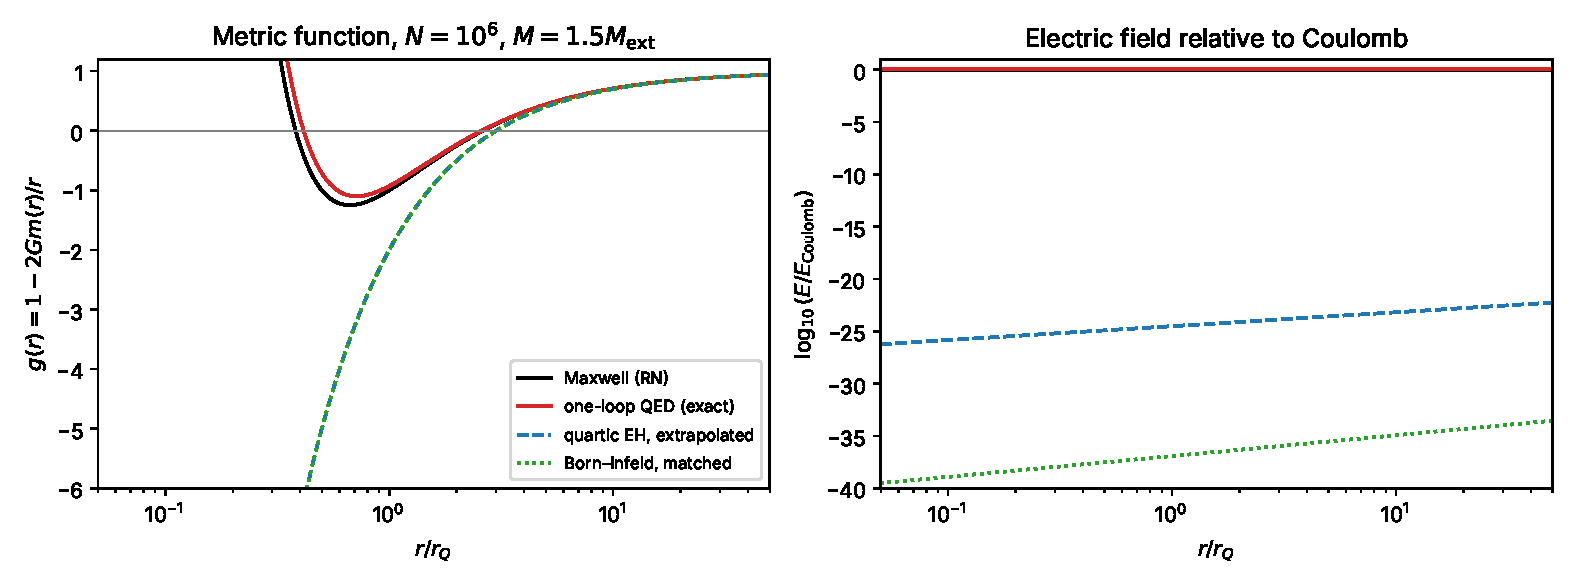
\includegraphics[width=0.92\textwidth]{fig_metric_profiles.pdf}
\caption{Metric function $g(r)=1-2Gm(r)/r$ (left) and electric field relative to Coulomb (right) for $N=10^6$ charges and $M=1.5M_{\rm ext}$, in the exact one-loop model, Maxwell (Reissner--Nordstr\"om), the quartic Euler--Heisenberg truncation extrapolated beyond its validity, and a Born--Infeld model matched to the quartic term.}
\label{fig:profiles}
\end{figure*}

\section{Trapping criterion derived inside the pipeline}\label{sec:trap}
The statement that the electrostatic energy does not help to trap a charged shell is standard in terms of the Misner--Sharp mass \cite{misner1964,hayward1994,boulware1973}; the charged Penrose inequality is a known theorem under stated hypotheses \cite{malec1994,khuri2017}. To remove any dependence on citations we derive what we use (gate \texttt{P10\_misner\_sharp\_symbolic}, ⟦branch_C.P10_n_parts⟧ sub-checks).

\emph{(a) Geometry.} In double-null coordinates, $ds^2=-2e^{2\sigma}du\,dv+R^2d\Omega^2$, with $M_{\rm MS}=(R/2G)(1-g^{ab}\partial_aR\,\partial_bR)$ and expansions $\theta_\ell=2\partial_uR/R$, $\theta_n=2\partial_vR/R$, SymPy proves
\begin{equation}
1-\frac{2GM_{\rm MS}}{R}=-\frac{R^2e^{-2\sigma}}{2}\,\theta_\ell\theta_n .
\end{equation}
Hence $\theta_+=0\Leftrightarrow2GM_{\rm MS}=R$ (for $\theta_-\neq0$), and a trapped surface is $2GM_{\rm MS}>R$.

\emph{(b) Constraint.} For time-symmetric data ($K_{ij}=0$) the Hamiltonian constraint follows from computing $G_{ab}n^an^b=2Gm'/r^2$ for a metric with arbitrary second time derivatives, which drop out; thus $m'=4\pi r^2\rho$. The radial Maxwell field obeys Gauss' law $r^2E_{\rm orth}=\mathrm{const}$ independently of the metric and $T_{ab}n^an^b=E_{\rm orth}^2/2$.

\emph{(c) ADM decomposition.} Integrating from $R$ to infinity,
\begin{equation}
M_{\rm ADM}=M_{\rm MS}(R)+U_C(R),\quad U_C(R)=\frac{Q^2}{8\pi R},
\end{equation}
so the exterior metric \emph{is} Reissner--Nordstr\"om, $g=1-2GM_{\rm ADM}/r+GQ^2/4\pi r^2$ (derived, not assumed).

\emph{(d) Cancellation.} At $\theta_+=0$, $GM_{\rm ADM}=(R+r_Q^2/R)/2$ with $r_Q^2=GQ^2/4\pi$ (the equality case of the charged Penrose inequality). With $M_{\rm MS}(R)=M_n$ the electrostatic term cancels identically: $G(M_n+U_C)-\tfrac12(R+r_Q^2/R)=GM_n-R/2$. Non-charged exterior matter with $\rho\ge0$ only adds mass, giving the inequality.

\textbf{Scope.} Proven in this subsection: spherical time-symmetric data, $\rho\ge0$, no charged matter outside the surface. The dynamical case ($K_{ij}\neq0$) is treated in Sec.~\ref{sec:dyn}; the persistence of trapped surfaces under $\mathrm{NEC}$ is cited, not proven. The control C4 verifies that wrong factors in $M_{\rm MS}$, in the constraint ($m'=2\pi r^2\rho$) or in $U_C$ are detected.

\emph{One-loop correction to $U_C$.} For a general $\mathcal L$ with $H(D)=ED-\mathcal L$ and $dH/dD=E$ (proved for arbitrary $\mathcal L$), $\rho=H(D)$, $D=a/r^2$, $a=Q/4\pi$, and
\begin{equation}
U(R)=2\pi a^{3/2}\!\int_0^{D_R}\!H(D)\,D^{-5/2}dD,\quad D_R=a/R^2 ,
\end{equation}
which gives $Q^2/8\pi R$ for Maxwell and $-16\pi c\,a^4/5R^5$ for the quartic term (symbolic). With the exact one-loop $H$ and $N=10^6$, $U_{\rm QED}/U_C-1=⟦#branch_C.U_QED.table.1e+00.delta_U|.3e⟧$ at $R=r_Q$, in agreement with a direct radial quadrature to ⟦#branch_C.U_QED.table.1e+00.rel_diff_direct|.1e⟧ (gate P11). The slope with respect to $\ln\eps$ is ⟦#branch_C.U_QED.slope_low|.4e⟧ ($\ln\eps\in[9,23]$) and ⟦#branch_C.U_QED.slope_dU_dlnx|.4e⟧ ($[18,60]$), approaching $\alpha/3\pi=⟦#branch_C.U_QED.slope_expected_alpha_over_3pi|.4e⟧$ with the $O(\alpha\ln\eps)$ sub-leading logarithm.

\subsection{Dynamical Misner--Sharp balance without time symmetry}\label{sec:dyn}
For the general metric $ds^2=-e^{2\phi(t,r)}dt^2+e^{2\lambda(t,r)}dr^2+r^2d\Omega^2$ and $M_{\rm MS}=(r/2G)(1-e^{-2\lambda})$, SymPy computes the full Einstein tensor and proves $G^t{}_t=-2GM_r/r^2$ and $G^r{}_t=2GM_t/r^2$, i.e.\
\begin{equation}
\partial_rM_{\rm MS}=4\pi r^2\rho,\qquad \partial_tM_{\rm MS}=4\pi r^2T^r{}_t=-4\pi r^2F_{\rm flux},\quad F_{\rm flux}\equiv-T^r{}_t ,\label{eq:msdyn}
\end{equation}
together with $K^r{}_r=-e^{-\phi}\partial_t\lambda=-4\pi Gre^{2\lambda-\phi}T^r{}_t$ and $K^\theta{}_\theta=0$ (D\_MS1): the slices have $K_{ij}\neq0$ if and only if there is an energy flux, so the data of gate P10 are exactly the zero-flux case. For a radial electric field (the Maxwell tensor is built from $F_{tr}=-e^{\phi+\lambda}E$, with $T^t{}_t=T^r{}_r=-E^2/2$, $T^\theta{}_\theta=E^2/2$ and $T^r{}_t=0$) SymPy verifies $\nabla_\mu T^\mu{}_\nu{}^{\rm (EM)}=F_{\nu\lambda}J^\lambda$ in the dynamical metric, with $J^\nu\equiv\nabla_\mu F^{\mu\nu}$, and that its $t$-component is $-\partial_t(E^2/2)$. If the plasma obeys $\nabla_\mu T^{\mu}{}_\nu{}^{\rm (pl)}=-F_{\nu\lambda}J^\lambda$, the two Einstein constraints $G^r{}_t$ and $G^r{}_r-G^t{}_t$ give
\begin{equation}
\partial_t\rho_{\rm tot}=\frac1{r^2}\partial_r\!\big(r^2T^r{}_t\big)\quad\text{independently of }F_{t\lambda}J^\lambda ,
\end{equation}
so the internal conversion $E^2/2\to\rho_{\rm pl}$ in $r<R$ conserves $M_{\rm MS}(t,R)$ exactly and $\partial_tM_{\rm MS}(t,R)=4\pi R^2T^r{}_t(R)$ depends only on the plasma flux through $r=R$ (D\_MS2); if the transfer law is altered to $(1+\delta)F_{t\lambda}J^\lambda$ a spurious volume source $4\pi\delta\!\int_0^Rr^2F_{t\lambda}J^\lambda dr$ appears (control C\_MS). For a boundary $r=R(t)$, $dM_{\rm MS}/dt=4\pi R^2(T^r{}_t+\dot R\rho)$ vanishes for comoving matter, so only the flux \emph{relative} to the surface matters (D\_MS3). Radial null streams $T^{\mu\nu}=\rho_\pm\ell_\pm^\mu\ell_\pm^\nu$ propagate with $v=\alpha/a=e^{\phi-\lambda}$ and, with $W_\pm=r^2\rho_\pm$,
\begin{align}
\partial_tW_++\partial_r(vW_+)&=-W_+\big[v(\phi_r+\lambda_r)+2\lambda_t\big],\label{eq:null1}\\
\partial_tW_--\partial_r(vW_-)&=+W_-\big[v(\phi_r+\lambda_r)-2\lambda_t\big],\label{eq:null2}
\end{align}
with $\lambda_t=-\tfrac12a^2v(W_+-W_-)/r$ and $\phi_r=\tfrac12a^2rp_r+(a^2-1)/2r$ ($8\pi G=1$ in these two expressions), where both the $t$ and $r$ components of $\nabla_\mu T^{\mu\nu}=0$ give the same equation (D\_MS4). Together with the conversion (field loses what the plasma gains) these equations preserve the momentum constraint, $r^2\partial_t\rho_{\rm tot}-\partial_r(r^2T^r{}_t)=0$ identically (D\_MS5); a statically ``held'' mass $\rho_{\rm mat}$ with $p=0$ violates it by the exact amount $4\pi Gr^4\rho_{\rm mat}v(\rho_--\rho_+)/(r-2GM)$, which is why $M_n$ is treated below as a test mass.

\emph{Initial data of a charged ball.} For a uniformly charged ball of radius $r_0$ with non-electromagnetic mass $M_n$, with $q\equiv r_Q/r_0$ and $C_n\equiv2GM_n/r_0$, the compactness profile outside the ball is $C(x)=[C_n+\tfrac65q^2-q^2/x]/x$, $x=r/r_0$ (interior field energy $q^2/5$, exterior $q^2$), whose maximum is $(C_n+\tfrac65q^2)^2/4q^2$. SymPy gives an apparent horizon already in the data when $C_n=0$ for $q\ge⟦branch_C2.P12.q_crit_Cn0|.4f⟧=5/3$, i.e.\ $r_0\le⟦branch_C2.P12.r0_over_rQ|.2f⟧\,r_Q$ (P12): this is the extremality bound $M_{\rm ADM}\ge Q$, and the discharge cannot undo it (NEC). The interior field energy of a ball, which does gravitate at the surface, is absent from the shell criterion $C_n=1$ used in Sec.~\ref{sec:phase}.

\section{Pair-plasma back-reaction}\label{sec:kinetic}
\subsection{Markov source up to the first zero}
For a homogeneous field $x(t)=eE(t)$ with local pair-creation rate $\Gamma(x)=x^2e^{-\pi/x}/4\pi^3$ (the $n=1$ Schwinger term, which is the \emph{mean pair number}; the vacuum-decay rate $2\,\mathrm{Im}\mathcal L_1$ contains the full series), conduction and polarization currents give
\begin{equation}
\dot x=-2e^2\Big[\!\int_0^t\!dt'\,\Gamma(x')\langle v\rangle+\Gamma(x)\frac{\langle m_\perp\rangle}{x}\Big],
\end{equation}
with $p(t,t')=\int_{t'}^tx$, $v=p/\sqrt{p^2+m_\perp^2}$ and $m_\perp^2=1+xs/\pi$ averaged over $s\sim\mathrm{Exp}(1)$. This is the Markov limit of the quantum Vlasov equation \cite{kluger1998,schmidt1998}. The first zero of the field occurs at $\tau_{\rm dis}=\kappa/(e\sqrt{eE_0})$ with $\kappa=⟦branch_B.scaling.kappa_inf|.4f⟧$ and exponent $⟦branch_B.scaling.tau0_exponent|.5f⟧$ (the exponent follows from scale invariance for $m\to0$, so only $\kappa$ carries information; it is specific to this model). The scheme is second order (observed order ⟦branch_B.convergence.order|.2f⟧) and an independent implicit-trapezoid solver agrees ($\tau_0=⟦branch_B.convergence.tau0_trap|.5f⟧$ vs ⟦branch_B.convergence.tau0.1|.5f⟧). As an order-of-magnitude check against a secondary report of Ref.~\cite{ruffini2010}, our first zero is $⟦audit_checks.ruffini_crosscheck.ours.10.tau0_first_zero.1|.3g⟧$ at $E_0=10E_c$ and $⟦audit_checks.ruffini_crosscheck.ours.0.15.tau0_first_zero.1|.2g⟧$ at $0.15E_c$ (in units of $\hbar/m_ec^2$), against $\sim10$ and $\sim10^7$ quoted there for an oscillation length; the definitions are not identical, so this is consistency, not validation.

\subsection{Pauli-blocked kinetics through repeated field reversals}
Removing the restriction to the first zero requires tracking occupation. We evolve $f(P,p_\perp,t)$ on a canonical-momentum grid with kinetic momentum $p=P+\Phi(t)$, $\dot\Phi=x$:
\begin{align}
\partial_tf&=(1-2f)\,S,\quad S=|x|e^{-\pi m_\perp^2/|x|}\,G_\sigma(p),\\
\dot x&=-2e^2\Big[\sum Wf\frac{p}{\omega}+\sum W\omega\,\frac{(1-2f)S}{x}\Big],\label{eq:kin}
\end{align}
with $\rho_{\rm pl}=2\sum Wf\omega$ and a Gaussian of width $\sigma=0.25\sqrt{\eps_0}$. SymPy proves that
\begin{equation}
\frac{d}{dt}\Big(\frac{x^2}{2e^2}+\rho_{\rm pl}\Big)=0
\end{equation}
holds identically \emph{only if} the polarization current carries the factor $(1-2f)$ (K1; the control C5 yields the residual $-4\omega Sf\neq0$ otherwise), and that the blocked equation has the exact solution $f=\tfrac12(1-e^{-2\int S})\in[0,\tfrac12)$ (K2).

\textbf{Results} (Fig.~\ref{fig:plasma}). Using an adaptive DOP853 integrator with zero-crossing detection over $\eps_0\in\{30,10^2,10^3,10^4\}$ we obtain at least $⟦branch_B2.sweep.100.n_cross⟧$ zero crossings (five full oscillations) with $\max|\Delta E|/E_0=⟦#branch_B2.sweep.10000.Emax_err|.1e⟧<10^{-4}$ (K5); $0\le f\le⟦branch_B2.sweep.100.fmax|.6f⟧$ everywhere (K4) whereas without blocking $f$ reaches $⟦branch_B2.pauli_effect_x100.f_max_noblock|.2f⟧>1$; without the blocking factor the model reproduces the cohort model of the previous subsection (K3, $\tau_0=⟦branch_B2.no_block_x100.tau0|.5f⟧$ vs $⟦branch_B.sweep.100.tau0|.5f⟧$), while blocking lengthens the first zero to ⟦branch_B2.pauli_effect_x100.tau0_block|.4f⟧ at $\eps_0=100$. The plasma frequency scales as $\omega_p\propto\eps_0^{⟦branch_B2.scaling.omega_exponent|.3f⟧}$ with $\omega_p=⟦branch_B2.scaling.omega_over_esqrtx0.2|.4f⟧\,e\sqrt{eE_0}$ (K7), and the amplitude decays slowly, $\gamma/\omega_p=⟦branch_B2.scaling.gamma_over_omega.2|.4f⟧$ (the amplitude falls from ⟦branch_B2.sweep.100.amps.0|.2f⟧ to ⟦branch_B2.sweep.100.amps.8|.2f⟧ of $E_0$ in nine half-cycles). Changing the tolerance, grid and transverse quadrature alters $\tau_0$ by at most ⟦#branch_B2.convergence.max_rel_change_tau0|.1e⟧ (K6); varying the source width within $[0.15,0.40]\sqrt{\eps_0}$ changes it by $⟦#branch_B2.sigma_sensitivity.max_rel_change_tau0|.1e⟧$. The negative controls (no $(1-2f)$ in $j_{\rm pol}$: $|\Delta E|/E_0=⟦branch_B2.controls.C6_energy_err|.1e⟧$ against ⟦branch_B2.sweep.100.Emax_err|.1e⟧ for the consistent model; $(1+2f)$: $f=⟦branch_B2.controls.C7_fmax|.0f⟧\gg\tfrac12$; wrong conduction sign) are all detected.

\textbf{Limitation.} A Markov equation with $S\ge0$ cannot raise $f$ above $\tfrac12$ from the vacuum, whereas the exact constant-field occupation $e^{-\pi m_\perp^2/\eps}$ exceeds $\tfrac12$ for $\eps>4.5$ and small $p_\perp$; for a single crossing the blocked rule gives $f=\tfrac12(1-e^{-2f_0})$, which is only ⟦branch_B2.single_crossing.ratio_at_f0_0p9|.2f⟧ of the exact value at $f_0=0.9$. The quantitative values of $\omega_p$ and $\gamma$ of this subsection are therefore properties of the Markov model; Sec.~\ref{sec:exact} replaces the ansatz by the exact kinetics \cite{schmidt1998,prakapenia2023} and quantifies the difference.

\begin{figure*}[t]
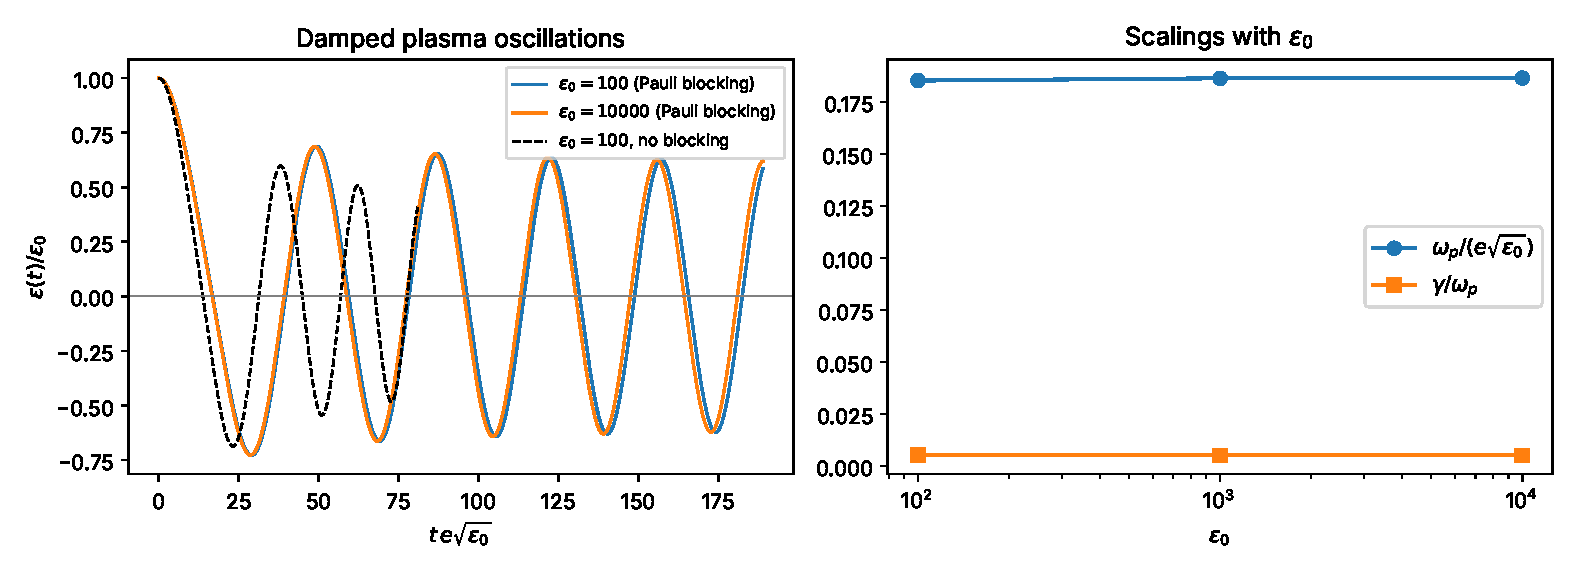
\includegraphics[width=0.92\textwidth]{fig_plasma_oscillations.pdf}
\caption{Left: electric field $\eps(t)/\eps_0$ in units of $1/(e\sqrt{\eps_0})$ for the Pauli-blocked Markov kinetic equation (solid) and without blocking (dashed), exhibiting the collapse of different $\eps_0$ onto one curve (scale invariance). Right: $\omega_p/(e\sqrt{\eps_0})$ and $\gamma/\omega_p$ as functions of $\eps_0$.}
\label{fig:plasma}
\end{figure*}

\subsection{Exact non-Markovian quantum kinetics}\label{sec:exact}
The Markov limit is removed by evolving, for every mode $(P,s{=}p_\perp^2)$ with kinetic momentum $p=P+\Phi(t)$, $\dot\Phi=x$ and $m_\perp^2=1+s$, the Bloch vector of the exact two-level Dirac problem $H=p\,\sigma_z+m_\perp\sigma_x$, with $f=(1-z)/2$, $u$ and $v$ the components of the Bloch vector along the adiabatic axes (Bloch--Bogoliubov form of the quantum Vlasov equation \cite{kluger1998,schmidt1998}):
\begin{align}
\dot f&=\tfrac12\lambda\,u,\quad \dot u=\lambda(1-2f)-2\omega v,\quad \dot v=2\omega u,\label{eq:bloch}\\
\dot x&=-2e^2\sum W\Big[\frac p\omega f+\frac{m_\perp}{2\omega}u\Big],\quad \lambda=\frac{x\,m_\perp}{\omega^2},\label{eq:maxw}
\end{align}
with $\omega=\sqrt{p^2+m_\perp^2}$, $\rho_{\rm pl}=2\sum W\omega f$ and the parallel pressure $P_\parallel=\sum Wp\,[2(p/\omega)f+(m_\perp/\omega)u]$ (Hellmann--Feynman). There is no source term, no locally-constant-field approximation and no source width: phase coherence between successive crossings and Pauli blocking are contained exactly. SymPy derives Eq.~\eqref{eq:bloch} from $\dot{\bf n}=2{\bf h}\times{\bf n}$ together with the velocity and energy identifications (Q0), proves that $\frac{d}{dt}[(1-2f)^2+u^2+v^2]=0$ identically, so that the vacuum $(0,0,0)$ implies $0\le f\le1$ without any truncation at $\tfrac12$ (Q1), proves $\frac{d}{dt}(x^2/2e^2+\rho_{\rm pl})=0$ with the polarization current of Eq.~\eqref{eq:maxw} (Q2; omitting it leaves the residual $W x\,m_\perp u/\omega\neq0$, control C10), and the trace identity $\rho_{\rm pl}-P_\parallel-2P_\perp=\sum W m^2(2f-pu/m_\perp)/\omega$ (Q4).

\textbf{Normalization of the coupling.} The form $\dot f=\lambda u$, $\dot u=2\lambda(1-2f)-2\omega v$ (the coupling of Eq.~\eqref{eq:bloch} doubled) is not excluded by the algebraic gates: it also conserves purity and energy (with a correspondingly doubled polarization current), so these gates cannot discriminate it, but it fails the Landau--Zener test: for $eE=10$, $m_\perp=1$ it gives $f_\infty=⟦branch_B3.landau_zener_literal_factor2.f_num.x10_eps2_1|.4f⟧$ instead of $e^{-\pi m_\perp^2/eE}=⟦branch_B3.landau_zener.x10_eps2_1.f_exact|.4f⟧$ (control C11). The coefficient of Eq.~\eqref{eq:bloch} is the one derived from the Dirac equation (Q0) and reproduces $f_\infty=e^{-\pi m_\perp^2/eE}$ to $⟦#branch_B3.lz_max_rel_err|.1e⟧$ or better in all $⟦branch_B3.n_lz_cases⟧$ test cases (Q3; the C kernel gives $⟦#branch_B3.kernel_lz.rel_err|.1e⟧$, Q3b), with $f_\infty$ up to $⟦branch_B3.lz_fmax|.3f⟧$, above the Markov ceiling $\tfrac12$ for $\eps>\pi/\ln2=⟦branch_B3.x_cross|.4f⟧$ (Q3a).

\textbf{Numerics.} A fixed-step RK4 scheme in C/OpenMP (time step $0.2/\omega_{\max}$, $P$-spacing $0.04\sqrt{\eps_0}$, 30 Gauss--Legendre nodes in $p_\perp^2$) integrates $⟦branch_B3.exact_sweep.100.N_modes⟧$ modes at $\eps_0=100$. The discrete system conserves $x^2/2e^2+\rho_{\rm pl}$ exactly, and the integrator preserves it to $⟦#branch_B3.max_energy_err|.1e⟧$ over at least five oscillations for $\eps_0\ge10$ (Q2b). Halving $\Delta P$ or $\Delta t$, doubling the transverse nodes or widening the $P$ range changes $\tau_0$ by $\le⟦#branch_B3.convergence.max_rel_change_tau0|.1e⟧$ and the first four half-periods by $\le⟦#branch_B3.convergence.max_rel_change_halfperiods_1to4|.1e⟧$ (K6); a narrow $P$ range is detected by the coverage gate (C12). The initial state is the zeroth-order adiabatic vacuum at $t=0$, as in the Markov model; replacing it with the first-order superadiabatic vacuum changes the first half-periods by $⟦#branch_B3.init_sensitivity.max_rel_change|.1e⟧$ (K8).

\textbf{Results} (Table~\ref{tab:exact}, Fig.~\ref{fig:exact}). The exact system is not capped at $\tfrac12$: $f_{\max}=⟦branch_B3.exact_sweep.100.fmax|.6f⟧$ at $\eps_0=100$ and $\ge⟦branch_B3.min_fmax_ge10|.5f⟧$ for every $\eps_0\ge10$ (Q1c), against $⟦branch_B3.markov_sweep.100.fmax|.4f⟧$ for the blocked Markov model; even at $\eps_0=4<\pi/\ln2$ interference between successive crossings reaches $f_{\max}=⟦branch_B3.exact_sweep.4.fmax|.4f⟧$. For a single crossing the blocked Markov rule undershoots by the fraction $⟦branch_B3.markov_single_crossing_deficit.at_f0_0p9|.3f⟧$ at $f_0=0.9$ (limit $⟦branch_B3.markov_single_crossing_deficit.limit_f0_1|.3f⟧$ for $f_0\to1$). The first zero of the field occurs earlier than in the Markov model: $\tau_0e\sqrt{\eps_0}=⟦branch_B3.exact_sweep.1000.tau0_e_sqrtx0|.2f⟧$ at $\eps_0=10^3$ against $⟦branch_B3.markov_sweep.1000.tau0_e_sqrtx0|.2f⟧$, a ratio $⟦branch_B3.comparison.1000.tau0_ratio_exact_over_markov|.3f⟧$ ($⟦branch_B3.comparison.10.tau0_ratio_exact_over_markov|.3f⟧$ at $\eps_0=10$, $⟦branch_B3.comparison.4.tau0_ratio_exact_over_markov|.3f⟧$ at $\eps_0=4$). The exact value is within $⟦branch_B3.tau0_vs_kappa_pct|.1f⟧$ per cent of the constant $\kappa=⟦branch_B.scaling.kappa_inf|.2f⟧$ of the unblocked source of Sec.~\ref{sec:kinetic}, so the lengthening attributed above to Pauli blocking is an artefact of the ceiling at $\tfrac12$. The plasma frequency (mean of the last three half-periods) scales as $\omega_p\propto\eps_0^{⟦branch_B3.scaling.omega_exponent|.3f⟧}$ with $\omega_p/(e\sqrt{\eps_0})=⟦branch_B3.scaling.omega_over_esqrtx0.3|.4f⟧$ for $\eps_0=10^3$, i.e.\ $⟦branch_B3.pct_omega_shift_1000|.1f⟧$ per cent above the Markov value $⟦branch_B3.scaling.omega_over_esqrtx0_markov.3|.4f⟧$ (K7). The amplitude decays slowly and non-exponentially (it falls from $⟦branch_B3.exact_sweep.1000.amps.0|.2f⟧$ to $⟦branch_B3.exact_sweep.1000.amps.5|.2f⟧$ of $E_0$ in six half-cycles), and the log-linear fit gives $\gamma/\omega_p=⟦branch_B3.scaling.gamma_over_omega.3|.4f⟧$ against $⟦branch_B3.comparison.1000.gamma_over_omega_markov|.4f⟧$; with ten amplitudes this number is a rough descriptor and the difference is not significant. \emph{Equation of state.} The total parallel $w_{\rm tot}=(P_\parallel-E^2/2)/(\rho_{\rm pl}+E^2/2)$ starts at $-1$ (pure field) and first reaches zero at $t\,e\sqrt{\eps_0}=⟦branch_B3.eos.1000.t_cross0|.2f⟧$ ($⟦branch_B3.eos.30.t_cross0|.2f⟧$ at $\eps_0=30$), before the first field zero at $⟦branch_B3.exact_sweep.1000.tau0_e_sqrtx0|.1f⟧$. The pairs themselves have $w_\parallel^{\rm pl}=P_\parallel/\rho_{\rm pl}>\tfrac13$ from the first instant ($t\,e\sqrt{\eps_0}\simeq⟦branch_B3.eos.100.t_third|.3f⟧$) and its average over the last period is $⟦branch_B3.exact_sweep.1000.w_pl_avg_last_period|.3f⟧$ (at most $⟦branch_B3.max_wpl|.3f⟧$ instantaneously, the excess over unity being the coherent term): it tends to the collinear value $1$, not to the isotropic $\tfrac13$, because the pairs are created with $p_\perp^2\sim\eps/\pi\ll p_\parallel^2$ and the homogeneous model has no collisions or transverse spreading that could isotropize them. \emph{Controls and sensitivity.} Without the polarization current the energy drifts by $⟦branch_B3.controls_C13_energy|.1e⟧$ (C13); with the doubled coupling (and a consistent doubled current) energy is conserved but $\tau_0e\sqrt{\eps_0}$ changes to $⟦branch_B3.literal_factor2_plasma.tau0_e_sqrtx0|.2f⟧$ (C14), so only Landau--Zener fixes the coefficient. The initial state is the zeroth-order adiabatic vacuum; the first-order superadiabatic vacuum changes $\tau_0$ by $⟦branch_B3.init_sensitivity.rel_change_tau0|.3f⟧$ of its value (K8).

\begin{table*}[t]
\caption{Exact (Bloch--Bogoliubov) versus Markov kinetics at the same $\eps_0$: maximum occupation, first zero $\tau_0e\sqrt{\eps_0}$, plasma frequency $\omega_p/(e\sqrt{\eps_0})$ (mean of the last three half-periods), $\gamma/\omega_p$ (log-linear fit of the half-cycle amplitudes), and the time-averaged parallel equation of state of the pairs over the last period. For $\eps_0=4$ only four zero crossings were computed.}
\label{tab:exact}
@@TABLE_EXACT@@
\end{table*}

\begin{figure*}[t]
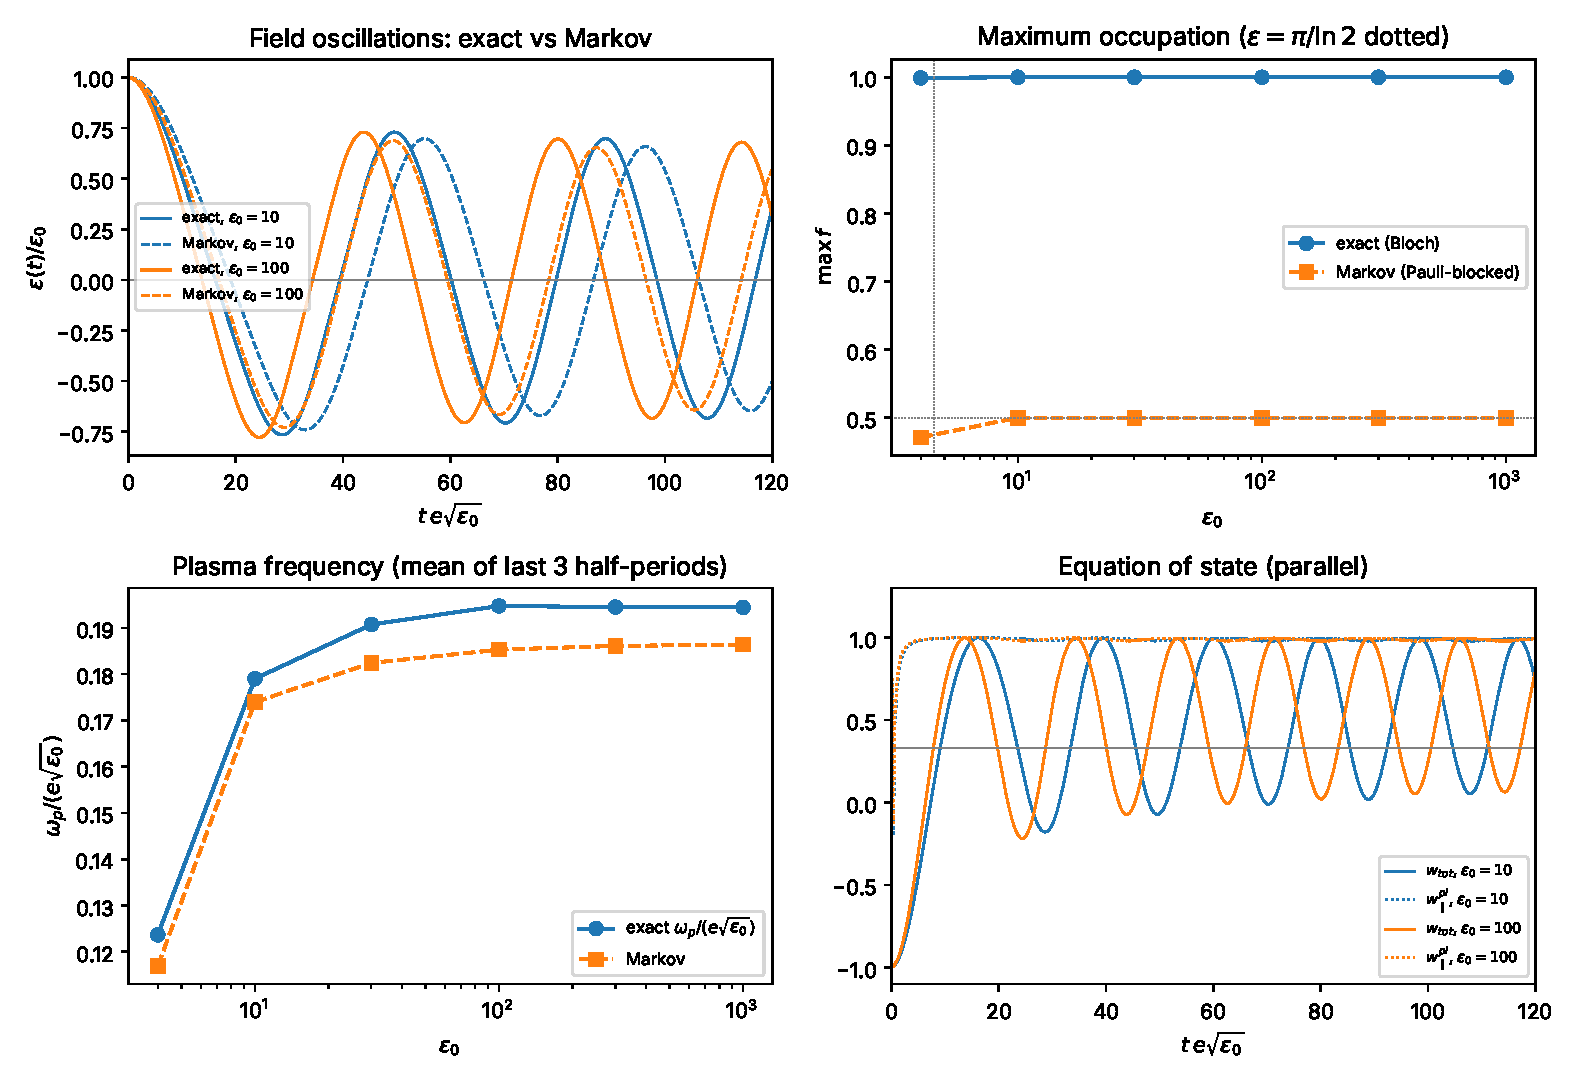
\includegraphics[width=0.92\textwidth]{fig_markov_vs_exact.pdf}
\caption{Exact non-Markovian quantum Vlasov (solid) versus the Pauli-blocked Markov model (dashed). Top left: field oscillations at $\eps_0=10$ and $100$. Top right: maximum occupation $f$; the exact system exceeds the Markov ceiling $\tfrac12$ above $\eps=\pi/\ln2$. Bottom left: plasma frequency. Bottom right: parallel equation of state $w_{\rm tot}=(P_\parallel-E^2/2)/(\rho_{\rm pl}+E^2/2)$ (solid) and $w_\parallel^{\rm pl}=P_\parallel/\rho_{\rm pl}$ (dotted).}
\label{fig:exact}
\end{figure*}

\section{Scales and phase map}\label{sec:phase}
For $N$ electrons of charge $Ne$ confined in radius $r_0$ (lengths in $\lC$): the field reaches $\eps=1$ at $r_\eps=\sqrt{N\alpha}$; the Reissner--Nordstr\"om radius is $r_Q=N\sqrt\alpha/\MPl$; the Coulomb density equals $\MPl^4$ at $r_P$ (with a floor of $10\,l_P$); and the trapping radius $r_s(N)$ solves $r=2G\,[N+\tfrac34(9\pi/4)^{1/3}N^{4/3}/r]$ (rest mass plus ultra-relativistic Fermi energy, gate P4). Because of the cancellation of Sec.~\ref{sec:trap}, $r_s$ is independent of the charge. The ratio of the electromagnetic to the gravitational force of the electron is $z^2=\alpha\MPl^2=⟦#branch_C.critical.z2_coulomb_over_gravity|.2e⟧$.

\textbf{Time scales.} With $E_0=Q/4\pi r_0^2$, $\eps_0=N\alpha/r_0^2$ and the result of Sec.~\ref{sec:kinetic}, $\tau_{\rm dis}=\kappa\,r_0/(\alpha\sqrt{4\pi N})$, equal to the light-crossing time at $N^*=\kappa^2/(4\pi\alpha^2)=⟦#branch_C.critical.N_star|.2e⟧$. For the free fall of a dust ball of mass $Nm_e$, $\tau_{\rm ff}=\tfrac\pi2\sqrt{r_0^3/2GM}$ (symbolic, P8). Both times scale as $N^{-1/2}$, so
\begin{equation}
\frac{\tau_{\rm dis}}{\tau_{\rm ff}}=\sqrt{\frac{r_0^*}{r_0}},\qquad r_0^*=\frac{2\kappa^2}{\pi^3\alpha^2\MPl^2}=⟦#branch_C.race_law.r0_star_over_lPlanck|.2e⟧\,l_P ,
\label{eq:ratio}
\end{equation}
independent of $N$ (gate P9). We stress that this closed form is the product of two power laws and of the electron's $z^2$; it only expresses that discharge is faster than free fall for every $r_0>l_P$ (since $r_0^*\ll l_P$ the value of $r_0^*$ itself lies outside the validity of either model). On the trapping boundary with the Fermi energy included, the discharge wins only for $N\gtrsim⟦#branch_C.critical.N_race_at_trap_boundary|.2e⟧$.

\textbf{Phase map} (Fig.~\ref{fig:phase}). Four regions: static EFT ($\eps<1$); Schwinger discharge ($r_P<r_0<r_\eps$ and untrapped); trapping ($r_0\le r_s$); and trans-Planckian. The trapped region always lies at $\eps\gg1$ and above the Planck floor for $N\gtrsim⟦branch_C.N_BH_min|.0f⟧$; a classical horizon enters the static-EFT region only for $N\gtrsim\alpha\MPl^4/4=⟦#branch_C.critical.N_classical_BH_in_EFT|.2e⟧$. The Coulomb density at $r_Q$ is $\rho/\MPl^4=1/(8\pi\alpha N^2)$ (P6), sub-Planckian for $N\ge$⟦branch_C.critical.N_P|.1f⟧. The ``trapping'' region $r_0\le r_s$ is the shell criterion $2GM_n\ge r_0$ (matter surface with no interior field energy); Sec.~\ref{sec:dyn1d} shows that for $N>N_A\simeq⟦#branch_C2.N_A_staticcurve_enters_initial_horizon|.1e⟧$ this curve lies inside the region $r_0\le0.6\,r_Q$ in which the initial data of a uniformly charged ball already contain an apparent horizon. Table~\ref{tab:scales} lists the scales. The electrons in region (ii) are not bound (the Coulomb energy exceeds the Fermi energy for $N\gtrsim⟦branch_C.critical.N_coulomb_over_fermi|.1e⟧$); $r_s$ is a condition on initial data, not a formation scenario.

\begin{figure*}[t]
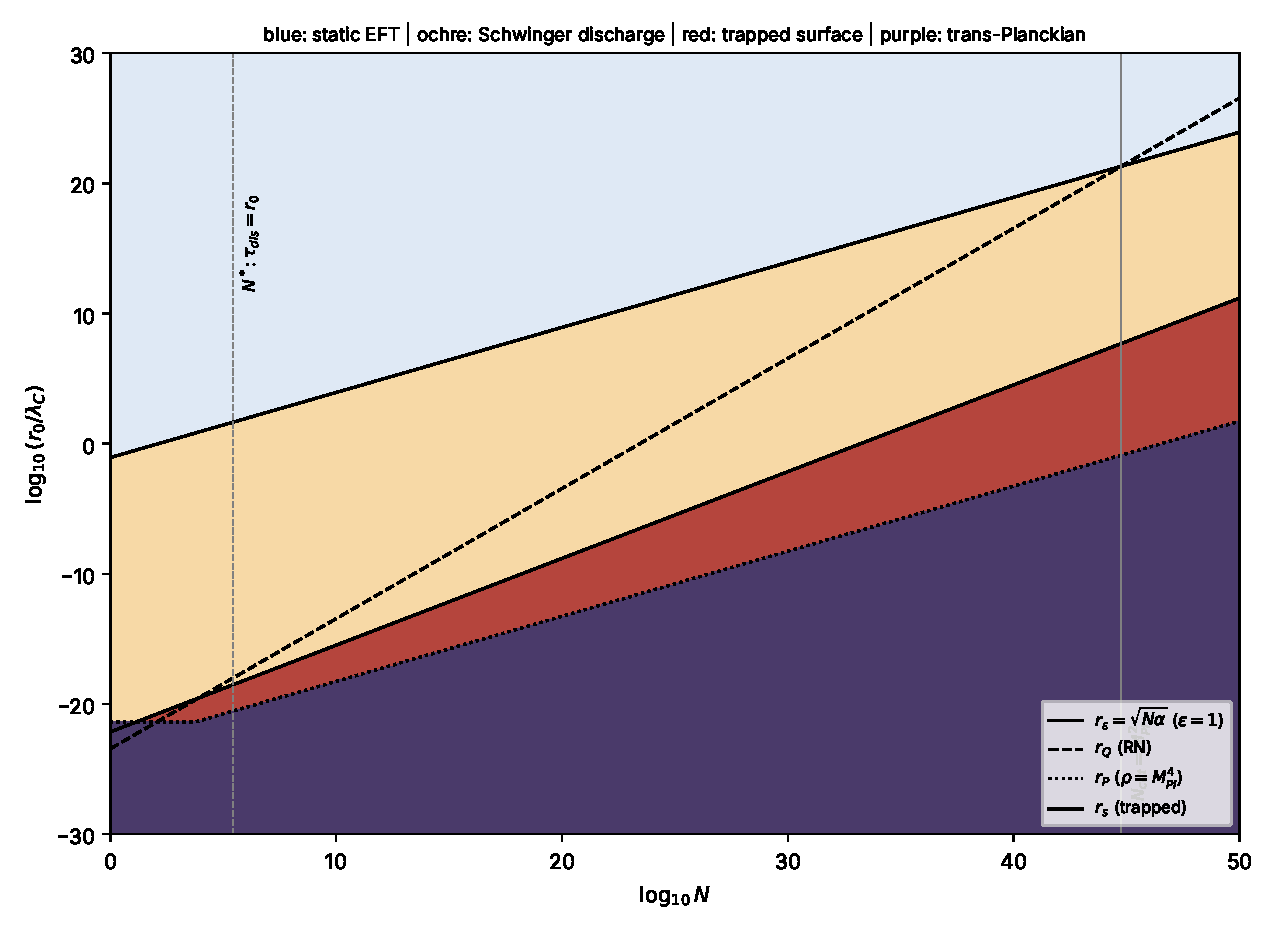
\includegraphics[width=0.78\textwidth]{phase_diagram.pdf}
\caption{Phase map in the $(N,r_0)$ plane. Solid lines: $r_\eps=\sqrt{N\alpha}$ and $r_s(N)$; dashed: $r_Q$; dotted: Planck-density radius. Vertical lines mark $N_{\rm crit}=\MPl^2/m_e^2$ and $N^*$ ($\tau_{\rm dis}=r_0$).}
\label{fig:phase}
\end{figure*}

\begin{table*}[t]
\caption{Characteristic radii (in $\lC$) and ratios for selected $N$ (computed in \texttt{06\_phase\_diagram.py}).}
\label{tab:scales}
\begin{ruledtabular}
@@TABLE_SCALES@@
\end{ruledtabular}
\end{table*}

\subsection{Spatially resolved discharge and trapping}\label{sec:dyn1d}
We evolve the system of Sec.~\ref{sec:dyn} on a radial grid in polar--areal gauge (script \texttt{06b\_dynamical\_trapping\_1d}; units $r_0=c=1$, $q=r_Q/r_0$, $s=\sqrt{N/N_*}$). The field of a uniformly charged ball, $\tilde\rho_{\rm EM}\propto q^2r^2$ ($r<1$) and $q^2/r^4$ ($r>1$), is converted locally with the clock $\dot s_c=\alpha\,\kappa s\sqrt{E/E_{\rm surf}}$ and the universal first-oscillation curve of the exact kinetics (Sec.~\ref{sec:exact}): the field decays as $E=E_{\rm geom}\,g(s_c)$ until its first zero, the energy removed is shared equally between an outgoing and an ingoing null stream (zero net momentum; the collinear plasma of Sec.~\ref{sec:exact} has $w_\parallel\simeq1$), and the metric follows from the constraints at every step. At the surface the discharge time is $r_0/s$ (so $s=1$ is $N=N_*$). The held mass $M_n$ enters as a static test mass. The flat limit with instantaneous discharge has a closed form, including the passage of ingoing rays through the centre: the solver reproduces $E_{\rm out}$ and $E_{\rm in}$ to $⟦#branch_C2.flat_limit.table.2000.err_out|.1e⟧$ and $⟦#branch_C2.flat_limit.table.2000.err_in|.1e⟧$ with observed order $⟦branch_C2.flat_limit.observed_orders.2|.2f⟧$ (N1; omitting the centre reflection gives an error of 3\%, control C\_N1). In the full theory the balance $m(r_0,t)-m(r_0,0)=\int(F_{\rm in}-F_{\rm out})dt$ of Eq.~\eqref{eq:msdyn} holds to $⟦#branch_C2.balance_summary.resmax|.1e⟧$ relative ($⟦#branch_C2.balance_summary.resabs|.1e⟧$ absolute) in ⟦branch_C2.balance_summary.n_cases⟧ cases with $q$ up to 1.3 (N2); a plasma that receives $1.2\times$ what the field loses breaks it by $⟦#branch_C2.control_no_balance.residual|.1e⟧$ (C\_N2). Grid convergence with $\Delta r$, $\Delta r/2$, $\Delta r/4$ is ⟦#branch_C2.convergence_summary.rel_final_max_consistent|.1e⟧ at most (N3).

\textbf{How much mass-energy leaves, and how much arrives.} Take weak gravity ($q=0.2$) and instantaneous discharge, evaluated at $t=r_0/c$ (perfectly radial streams form a central caustic after that time; beyond it, up to the free-fall time $\tfrac\pi2r_0$ of the trapping boundary, a reflecting core of radius $r_{\rm core}=⟦branch_C2.threshold_response.r_core|.1f⟧\,r_0$ stands in for the angular momentum of the rays, $\theta_\perp\simeq\sqrt{1-w_\parallel}\simeq0.11$ from Sec.~\ref{sec:exact}; it conserves energy exactly, $|\Delta m-\!\int\!F|\le⟦#branch_C2.core_summary.balance_abs_max|.1e⟧$, changes $\Delta C$ by ⟦branch_C2.core_summary.core_variation_q0p5|.3f⟧ for $r_{\rm core}=0.05\to0.2$ at $q=0.5$ and by $⟦#branch_C2.core_summary.core_variation_q1|.1e⟧$ at $q=1$, N10). A neutral matter element released from rest follows the radial geodesic of the evolving metric; in a point-mass test its proper fall time agrees with the exact cycloid to $⟦#branch_C2.geodesic_vs_schwarzschild.0.rel_err|.1e⟧$ (N9), which validates $\alpha$, $a$, $\phi_r$ and $\lambda_t$ used for the dynamics. The interior channel (field energy inside the ball converted into plasma that crosses $r_0$ outwards) removes $\Delta C=⟦branch_C2.weak_gravity_F.inst.interior_only|.4f⟧\,q^2$ from $C=2GM_{\rm MS}(r_0)/r_0$, i.e.\ a fraction $⟦branch_C2.weak_gravity_F.inst.f_esc_interior|.3f⟧$ of the interior field energy ($⟦branch_C2.weak_gravity_F.1.0.f_esc_interior|.3f⟧$ for $s=1$) and $⟦branch_C2.loss_fraction_of_UC|.3f⟧$ of the total field energy $U_C$. The exterior channel (field energy outside the ball converted in place, whose ingoing half enters $r_0$) adds $⟦branch_C2.weak_gravity_F.inst.exterior_only|.4f⟧\,q^2$, $⟦branch_C2.inflow_over_leak|.2f⟧$ times larger, so the net effect is a \emph{gain}, $\Delta C=+⟦branch_C2.weak_gravity_F.inst.both|.4f⟧\,q^2$: the quasilocal mass at the surface is increased, not decreased, by the discharge. The net gain depends on the discharge speed as $\Delta C\simeq q^2F_\infty s^p/(s^p+s_h^p)$ with $F_\infty=⟦branch_C2.F_scaling.F_inf|.4f⟧$, $p=⟦branch_C2.F_scaling.hill_p|.2f⟧$, $s_h=⟦branch_C2.F_scaling.hill_s_half|.2f⟧$ (N4, N8): it is the instantaneous-discharge value for $N\gg N_*$ and falls as $s^{p}$ for $N\ll N_*$, where the plasma escapes ballistically before the field is converted ($⟦branch_C2.weak_gravity_F.0.3.both|.4f⟧\,q^2$ at $s=0.3$). Gravity suppresses the inflow: at $q=1$, $\Delta C/q^2=⟦branch_C2.strong_gravity.1.0.inst|.3f⟧$ (instantaneous) and at $q=1.5$ it is $⟦branch_C2.strong_gravity.1.5.inst|.4f⟧$, and a held mass $C_n=0\to0.6$ lowers $\Delta C$ at $q=1$, $s=3$ from $⟦branch_C2.Cn_dependence_q1_s3.0.0|.4f⟧$ to $⟦branch_C2.Cn_dependence_q1_s3.0.6|.4f⟧$, because the coordinate speed $v=\alpha/a$ vanishes as $\theta_+\to0$ (N5).

\textbf{Displacement of the trapping threshold.} Just below the static horizon threshold of P12, at $C_n=C_n^{\rm AH}(q)-⟦branch_C2.threshold_response.offset_below_threshold|.2f⟧$ with $C_n^{\rm AH}=1-q^2/5$ for $q<1$ and $2q-\tfrac65q^2$ for $q\ge1$, the maximum of the compactness profile grows by at most $\delta C_n=⟦branch_C2.threshold_response.delta_Cn_max|.4f⟧$ until $t=r_0/c$ and $⟦branch_C2.threshold_response.delta_Cn_max_ff|.4f⟧$ until the free-fall time $\tfrac\pi2r_0$, over $q\in[0.3,1.5]$ and $s\in[0.1,\infty)$ ($⟦branch_C2.threshold_response.delta_Cn_max_s1_ff|.4f⟧$ at $s=1$); no case forms a new horizon, and the numerical initial compactness reproduces the closed form to $⟦#branch_C2.threshold_response.max_Cmax0_discretization_err|.1e⟧$ (N6). Therefore the dynamics shifts the critical non-electromagnetic mass, $\Delta M_{\rm crit}/M_{\rm crit}$, by at most $⟦branch_C2.threshold_response.delta_Cn_max_ff|.4f⟧$ ($⟦branch_C2.threshold_range_pct|.1f⟧$\%) within the free-fall time, and in no regime does the escaping plasma delay trapping: the effect that dominates the retained mass is the \emph{static} interior field energy $q^2/5$, which the shell criterion of Sec.~\ref{sec:phase} omits. Figure~\ref{fig:dyntrap} shows the resulting curves in the $(N,r_0)$ plane: the horizon boundary $r_{\rm AH}(N)$ of the ball (P12 plus dynamics) lies above the shell curve $r_s(N)$ by a factor up to $⟦branch_C2.curve_summary.ratio_AH_over_rs_max|.0f⟧$ for $N\le10^{14}$, the two cross at $N_A\simeq⟦#branch_C2.N_A_staticcurve_enters_initial_horizon|.2e⟧$ (where $r_s=0.6r_Q$), and the dynamic correction is $r^{\rm dyn}/r_{\rm AH}-1\le⟦#branch_C2.curve_summary.rel_shift_dyn_vs_AH_max|.1e⟧$. For $N>N_A$ the curve $r_s(N)$ of the previous sections lies \emph{inside} the region where the initial data already contain an apparent horizon; there the race between discharge and free fall (Eq.~\eqref{eq:ratio}) is moot, because discharge cannot remove a trapped surface that already exists.

\begin{figure*}[t]
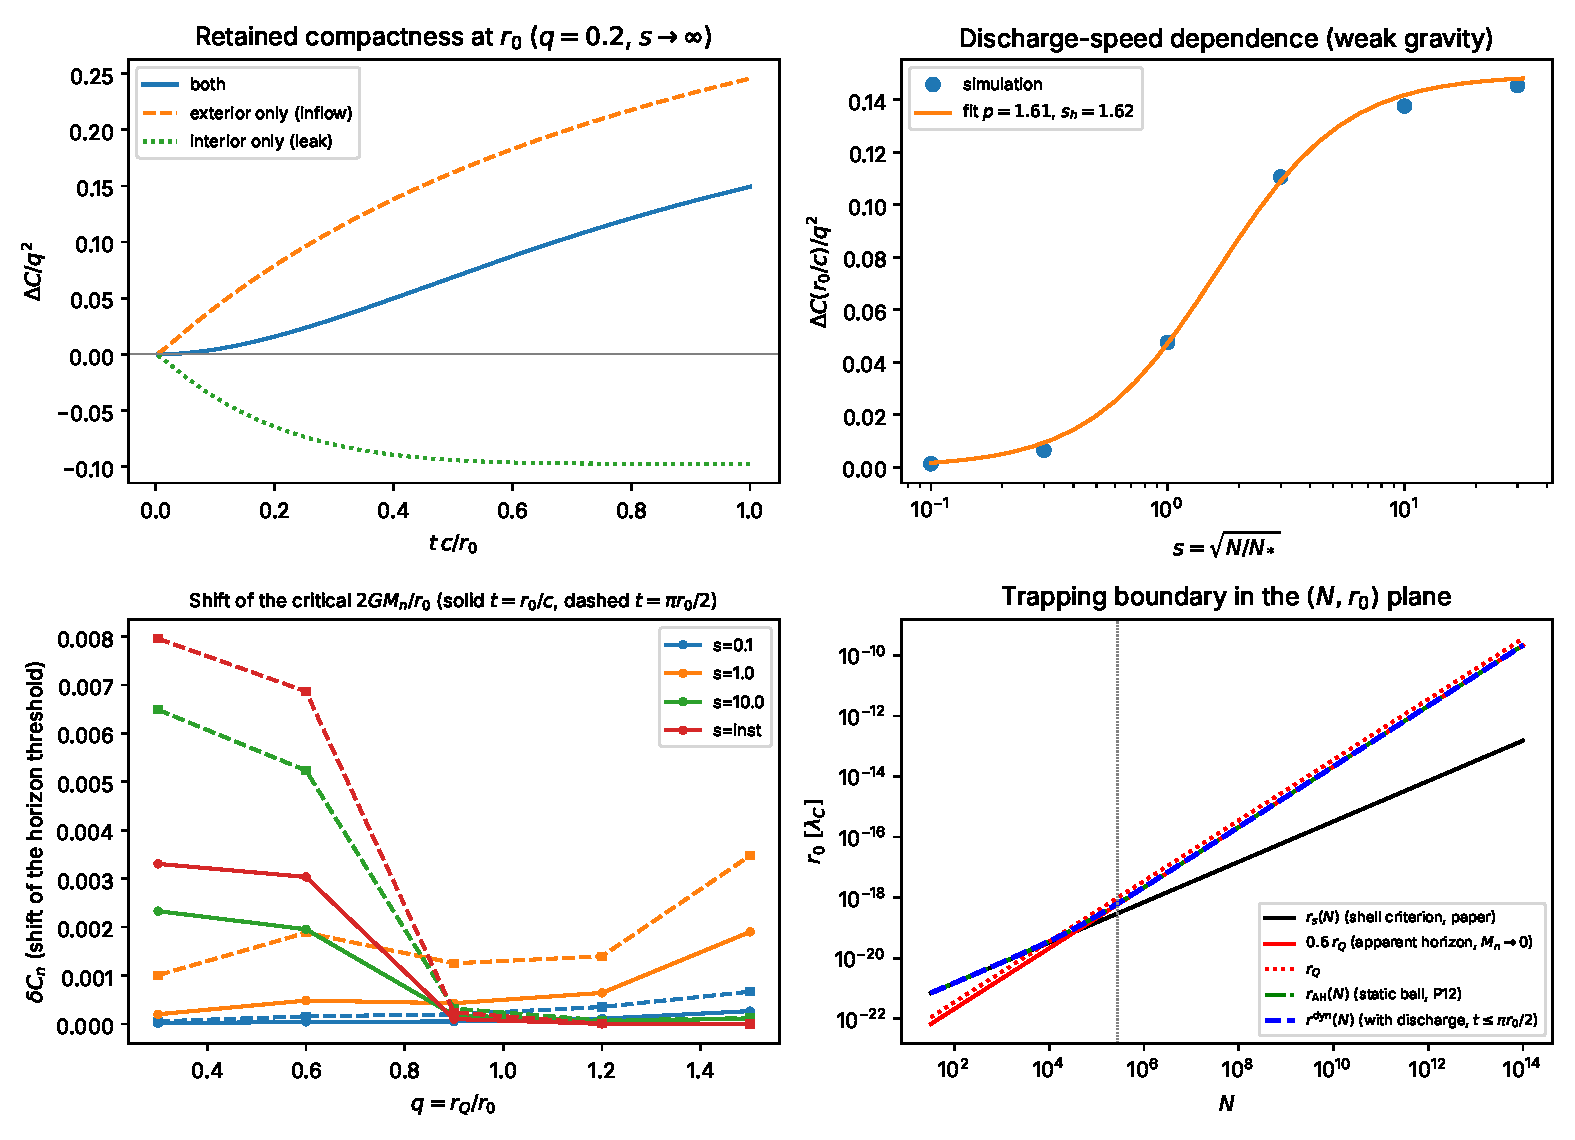
\includegraphics[width=0.92\textwidth]{fig_dynamic_trapping.pdf}
\caption{Spatially resolved discharge. Top left: retained compactness at $r_0$ for the interior (leak), exterior (inflow) and combined channels ($q=0.2$, instantaneous discharge). Top right: dependence on $s=\sqrt{N/N_*}$ and fit. Bottom left: shift $\delta C_n$ of the critical $2GM_n/r_0$ produced by the dynamics (solid: $t=r_0/c$; dashed: $t=\pi r_0/2$ with a reflecting core). Bottom right: boundaries in the $(N,r_0)$ plane: shell criterion $r_s$, $r_Q$ and $0.6\,r_Q$, apparent-horizon boundary of the static ball $r_{\rm AH}$ and the corrected curve $r^{\rm dyn}$ (indistinguishable from $r_{\rm AH}$ at this scale).}
\label{fig:dyntrap}
\end{figure*}

\begin{figure}[t]
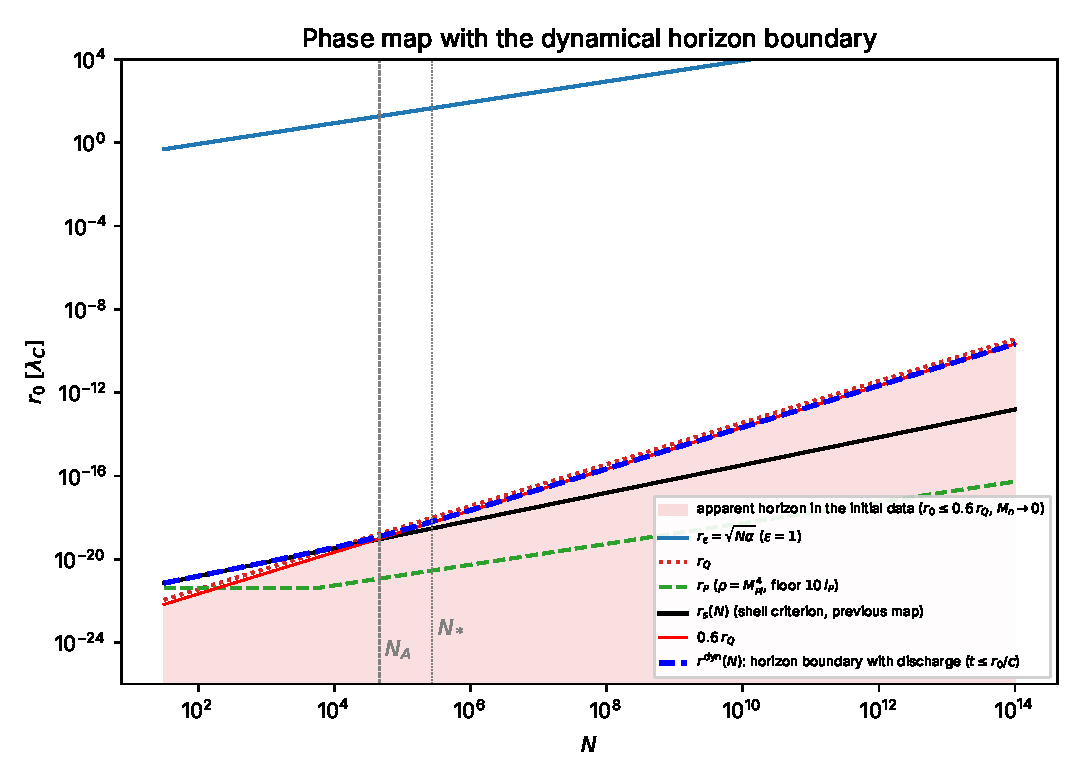
\includegraphics[width=\columnwidth]{phase_diagram_corrected.pdf}
\caption{Phase map of Fig.~\ref{fig:phase} with the horizon boundary of the charged ball: the shaded region has an apparent horizon in the initial data for arbitrarily small $M_n$; the curve $r^{\rm dyn}(N)$ includes the discharge up to $t=\pi r_0/2$ and coincides with $r_{\rm AH}$ to $10^{-3}$. For $N>N_A$ the shell curve $r_s$ lies inside the shaded region.}
\label{fig:phasecorr}
\end{figure}

\section{What is known and what is specific to this work}\label{sec:attrib}
\begin{table*}[t]
\caption{Attribution of the results. ``Known'' means that the mathematical structure was published before; ``here'' lists what the pipeline adds.}
\label{tab:attrib}
\begin{tabular}{p{4.2cm}p{5.2cm}p{7.2cm}}\toprule
Result & Prior work & Contribution of this work\\\midrule
Coulomb energy cancels in trapping & Misner--Sharp mass with charge, thin-shell energy equation, charged Penrose inequality \cite{misner1964,hayward1994,boulware1973,malec1994,khuri2017} & Derivation inside a CAS under explicit hypotheses (time-symmetric data, $\rho\ge0$, no exterior charge); one-loop-exact $U_C(R)$\\
Plasma oscillations, Markov source, $\omega_p\propto e\sqrt{eE}$ & \cite{kluger1991,kluger1992,kluger1998,schmidt1998,ruffini2010,gelis2016} & Exact energy identity with $(1-2f)$ in $j_{\rm pol}$, $f\le\tfrac12$, constants $\omega_p$, $\gamma$ for this source; convergence and negative controls\\
Bloch--Bogoliubov quantum Vlasov with Maxwell back-reaction & \cite{kluger1998,schmidt1998,prakapenia2023} & Same equations (a rediscovery); here: symbolic Dirac$\to$Bloch derivation, a Landau--Zener test that fixes the normalization of the coupling, a like-for-like Markov--exact comparison ($\tau_0$, $\omega_p$, $\gamma$, $f_{\max}$) and the parallel equation of state; not compared with published curves\\
Strong-field logarithm, Landau scale & \cite{ritus1975,dunne2004} & Exact evaluation of the electric proper-time integral and the constant $K$\\
DEC violation & One-loop trace anomaly \cite{adler1977,collins1977} & Exact onset $\eps=$⟦branch_A.energy_conditions_qed.DEC_onset_eps_exact|.5f⟧ and identity $x^3(\mathcal L_1/x^2)'$\\
Dynamical Misner--Sharp equations, quasilocal flux balance, radial null-dust transport in polar--areal gauge & \cite{misner1964,hayward1994} (standard) & Derivation in a CAS for the general $\phi(t,r),\lambda(t,r)$ metric with a Maxwell field and an exchange term, negative control for the transfer law; the conclusion that field$\to$plasma conversion inside $R$ conserves $M_{\rm MS}$ and only the surface flux counts is classical\\
Channel decomposition (leak from inside, inflow from outside) and its dependence on $q$ and $N/N_*$ & none found; radiation collapse of null shells is classical & Quantitative numbers for this specific discharge closure; not a prediction (closure ansatz, test-mass matter, radial beams)\\
Discharge of charged black holes, $N_{\rm crit}$ & Gibbons \cite{gibbons1975} & Reformulation of the scale in the $(N,r_0)$ plane\\
EH black holes (quartic) & \cite{yajima2001,ruffini2013} & Quantitative comparison with the exact one-loop interior in the coupled system, with explicit limits of validity\\
$\tau_{\rm dis}/\tau_{\rm ff}=(r_0^*/r_0)^{1/2}$, phase map & Elementary combination of known scalings & Closed forms with $\kappa$, verified symbolically; organization in one plane\\\bottomrule
\end{tabular}
\end{table*}

\section{Regimes where the model is not controlled}\label{sec:limits}
(1) \emph{Higher loops.} All strong-field statements are one-loop; Ritus--Narozhny scaling may invalidate them for $\eps\gtrsim10^3$--$10^6$. The sweep of the kinetic model reaches $\eps_0=10^{10}$, ⟦#audit_checks.orders_above_RN_threshold_in_05|.1f⟧ orders above that threshold. (2) \emph{Derivative expansion and curvature.} The profiles of Sec.~\ref{sec:static} descend to $r\sim10^{-18}\lC$; the curvature couplings of the one-loop action \cite{drummond1980} are of relative order $\alpha(\lC/L)^2$ and are neglected, and the local-field Lagrangian is not controlled there. (3) \emph{Imaginary part.} For $\eps>1$ the vacuum-decay rate is $O(1)$ and the real part alone is not a stable effective action. (4) \emph{Kinetics.} The exact Bloch system of Sec.~\ref{sec:exact} has no LCFA and no $f\le\tfrac12$ cap, but it is homogeneous, has no collisions or spatial transport (the pairs do not isotropize: $\langle w_\parallel\rangle\simeq1$), starts from the zeroth-order adiabatic vacuum (a ⟦#branch_B3.init_sensitivity.max_rel_change|.1e⟧ effect on the half-periods), uses a finite $(P,p_\perp)$ quadrature (converged to ⟦#branch_B3.convergence.max_rel_change_halfperiods_1to4|.1e⟧), and only reaches $\eps_0=10^3$; the Markov constants of Sec.~\ref{sec:kinetic} are model-specific, and the first-zero scale $\kappa$ of the cohort model (LCFA, Markov, $t_{\rm form}/\tau_0\simeq e/\kappa=⟦branch_B.scaling.lcfa_e_over_kappa|.3f⟧$) agrees with the exact kinetics only to the ⟦branch_B3.tau0_vs_kappa_pct|.1f⟧ per cent quoted in Sec.~\ref{sec:exact}. (5) \emph{Dynamics of trapping.} The dynamical Misner--Sharp balance is proven (Sec.~\ref{sec:dyn}) and the 1+1D solver is validated (flat limit, balance, convergence, geodesic test), but the collapse race is not evolved self-consistently: the time available for trapping is the \emph{prescribed} free-fall time $\tfrac\pi2r_0$ of the trapping boundary, and the matter $M_n$ is held at $r_0$ as a static test mass (its constraint violation is ⟦#branch_C2.held_matter_systematic.0.rel_gap|.2f⟧--⟦#branch_C2.held_matter_systematic.2.rel_gap|.2f⟧ of $\Delta C$ in the cases tested); a moving charged shell would also need its radial stress (the lapse jumps across it) and the Coulomb force on its carriers, neither of which is modelled. The plasma is a set of radial null streams whose central caustic is regularized by a reflecting core ($r_{\rm core}=0.1r_0$); the local discharge law is the homogeneous kinetics of Sec.~\ref{sec:exact} applied cell by cell, Gauss's law is not imposed during the conversion, and collisions, transverse spreading and the Coulomb explosion of the charge carriers are not included. The polar--areal gauge fails once an apparent horizon forms, so no evolution beyond that point is claimed. (6) \emph{Landau and Planck.} The Landau pole and the Planck density are never crossed in any calculation; the Planck floor defines region (iii) and no statement is made there.

\section{Conclusions}\label{sec:concl}
Beyond the point where the quartic static EEH description fails, the exact one-loop static field does not saturate and does not censor the horizon; the electrostatic energy \emph{outside} the surface plays no role in the trapping of that surface, which for a shell requires non-electromagnetic mass, $GM_n\ge R/2$ (the interior field energy of a ball does gravitate, Sec.~\ref{sec:dyn}); and pair discharge converts the field into plasma on the time $\tau_{\rm dis}=\kappa/(e\sqrt{eE_0})$ while conserving energy-momentum, so it cannot remove mass or undo a trapped surface. In the exact homogeneous kinetics the resulting collinear pair plasma oscillates for many periods with $\omega_p\simeq⟦branch_B3.scaling.omega_over_esqrtx0.3|.3f⟧\,e\sqrt{eE_0}$ (the Pauli-blocked Markov model gave ⟦branch_B2.scaling.omega_over_esqrtx0.2|.3f⟧), reaches occupations up to unity, and has $\langle w_\parallel\rangle\simeq1$. What discharge does remove is the net charge whose repulsion exceeds gravity by $z^2\sim10^{42}$, and it does so faster than free fall. These conclusions are consistent with the classical picture of Misner--Sharp, Boulware and Gibbons; the added value of this work is a verified quantitative map of where each description holds, together with an open, reproducible pipeline. Collisional isotropization, a comparison with published non-Markovian curves and the evolution of the matter and of the plasma beyond the first light-crossing time (central caustic, formation of the horizon) remain open. For the spatial and gravitational gap, the complete Misner--Sharp balance with $K_{ij}\neq0$ is derived, the discharge of a charged ball is simulated, and the result is that the dynamics moves the horizon threshold by less than ⟦branch_C2.threshold_range_pct|.1f⟧ per cent up to the prescribed free-fall time while the static interior field energy, absent from the shell criterion, relocates the threshold to $r_0\simeq0.6\,r_Q$ for large $N$.

\begin{acknowledgments}
The symbolic derivations, code and first draft of the text were produced with an AI assistant (Claude, Anthropic) operating the open pipeline described in Appendix~\ref{app:pipeline}; the author is responsible for the content. Bibliographic details marked in \texttt{references.bib} must be verified against the original publications before submission.
\end{acknowledgments}

\appendix
\section{Verification pipeline and reproducibility}\label{app:pipeline}
The repository (\url{https://github.com/lopezalmeidaalvaro/experimento}) contains numbered scripts executed by \texttt{run\_all.sh}, which stops at the first failing gate. Symbolic gates assert $\mathrm{simplify}(\mathrm{LHS}-\mathrm{RHS})=0$; numerical gates include convergence under refinement and an independent method; negative controls assert that altered signs, factors or conservation laws are detected. The totals are ⟦meta.n_gates⟧ gates, of which ⟦meta.n_negative_controls⟧ are negative controls. Table~\ref{tab:gates} lists the gates by script.
@@GATE_TABLE@@

\bibliography{references}
\end{document}
